\section{Introduction}
\label{sec:introduction}

Elephant Agent starts from the animal before the architecture. Elephant memory
is not merely large storage. Elephants recognize herd members, remember danger
cues, return to important locations after long gaps, and preserve bonds with
other animals and humans over years. Their hippocampus links emotion to
long-term memory, while their cerebral cortex supports problem solving,
cooperation, tool use, and simple quantitative tracking. In older matriarchs,
memory can become practical judgment for the herd: a remembered drought, route,
or warning sign changes future behavior.

Personal AI has an analogous design problem. It is not only an assistant that
can answer the current prompt. It is an individual system that should become
better at working with a particular person across days, surfaces,
interruptions, corrections, and repeated work. The central improvement target
is therefore not a larger chat window, a longer log, a vector memory store, or
a growing catalog of reusable skills. The central target is the Personal Model:
the explicit object that says what the agent currently understands about the
person, why it believes that, what is uncertain, and what should be asked next.

This distinction matters because many personal-agent systems now include
memory, and many self-evolving agent systems define progress primarily as
acquiring reusable skills, tools, or automations. Those capabilities are
valuable, but they answer different questions. Raw recall asks what can be
retrieved from the past. Skills ask what the agent can do. Personal AI also
needs to answer what it currently understands about the person and how that
understanding should change. Elephant Agent places this third object at the
center. Memory is not discarded or narrowed to retrieval; retrieval becomes one
layer in an architecture that turns episodes, relationships, risk patterns, and
background reflection into correctable understanding. Capabilities can then be
selected as operator-managed tools, but durable personalization remains in
correctable facts, open questions, and source provenance rather than hidden
skill weights or nearest-neighbor notes.

Elephant Agent implements this Personal-Model-first approach as a personal AI runtime
with durable continuity. It records atomic events as Steps, binds them to
execution Loops, groups Loops into Episodes, keeps Elephant State deliberately small,
and evolves the Personal Model through foreground updates, proactive questions,
and background reflect jobs. The clean product-facing memory architecture has
five layers:

\begin{center}
\texttt{Personal Model -> Elephant State -> Step Trail -> Contextual Recall -> Background Learning}
\end{center}

\begin{figure}[t]
  \centering
  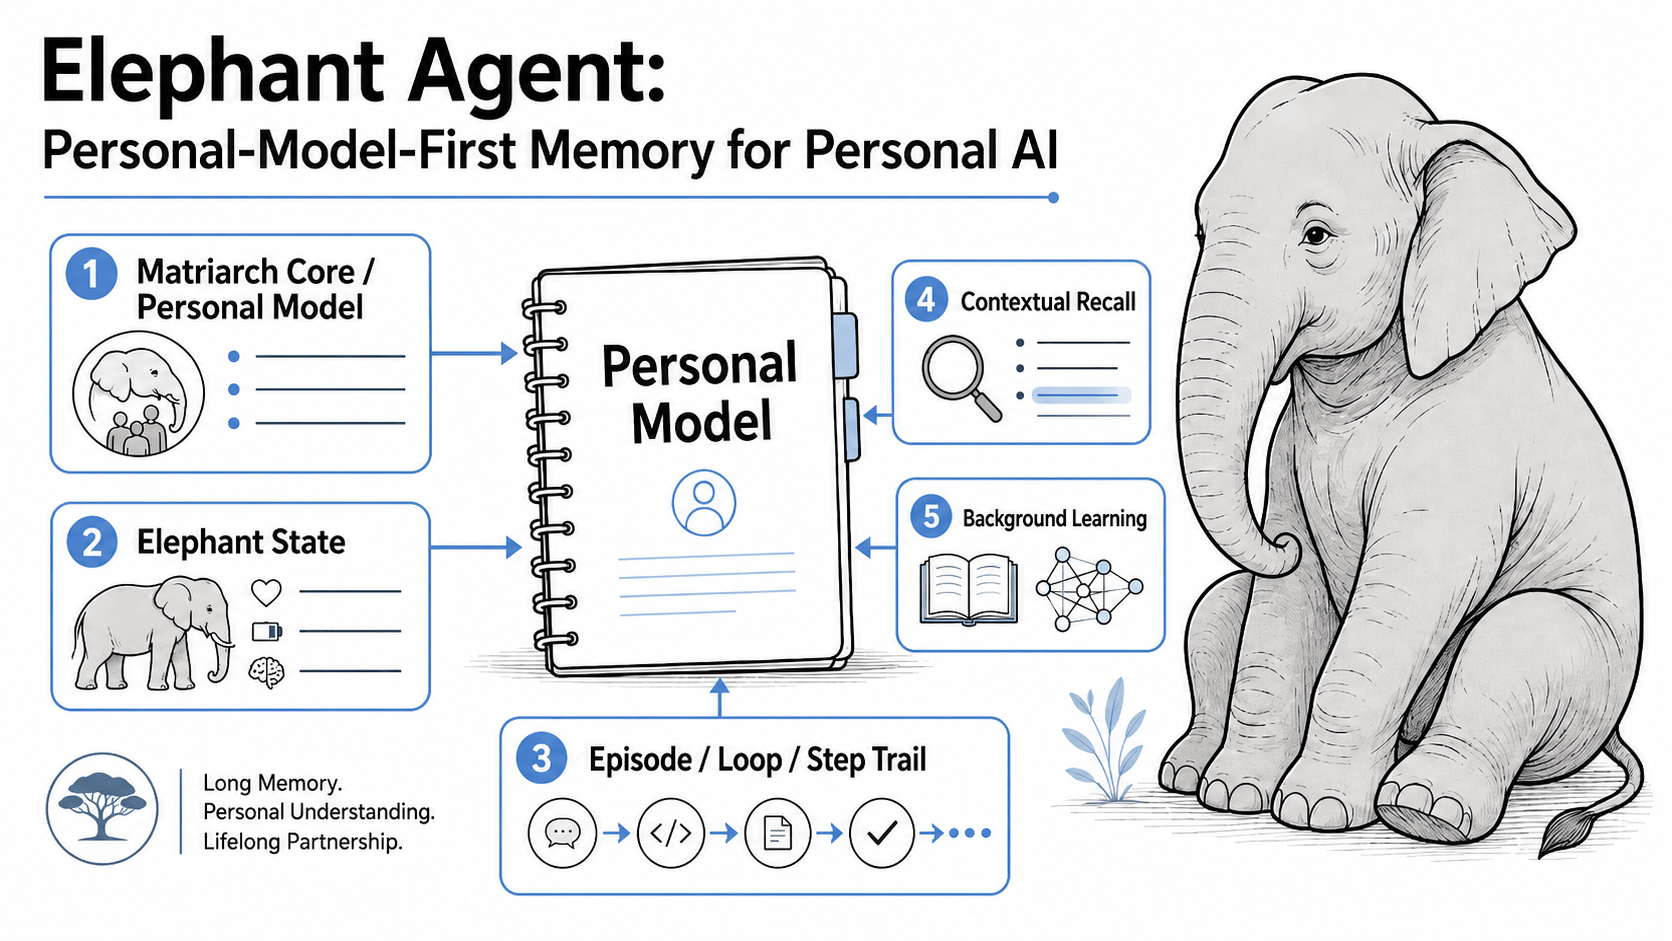
\includegraphics[width=\linewidth]{../../apps/site/static/assets/resources/paper-1.png}
  \caption{Elephant Agent centers personal AI evolution on a correctable
  Personal Model rather than on transcript accumulation or skill growth alone.}
  \label{fig:personal-model-overview}
\end{figure}

The Personal Model is the durable understanding layer. Elephant State carries the
Elephant Agent identity and one natural-language current context note. An Episode is one
wake or open runtime window. A Loop is one model interaction round. A Step is
one atomic event inside a Loop. Together they form the Episode / Loop / Step
trail. Contextual Recall retrieves support from Steps and Facts for the current
turn or a reflect job. Background Learning decides when evidence should change
claims or questions. Steps are the evidence; facts carry their own source
Episode provenance.

This report describes Elephant Agent as a system, not as an implementation plan. The
runtime provides six practical capabilities:

\begin{enumerate}[leftmargin=*]
  \item \textbf{Elephant-based continuity.} Elephant Agent resumes from a durable elephant rather
  than treating a session, thread, or transcript as the owner of continuity.

  \item \textbf{Personal Model evolution.} Long-term user understanding is
  represented as active four-lens facts with confidence, source episodes,
  correction, and governance.

  \item \textbf{Proactive curiosity.} The system can ask at quiet, balanced, or
  active effort levels when a gap, conflict, stale Pulse, or adaptation would
  materially improve future help.

  \item \textbf{Claim-aware recovery.} Explicit user-directed updates change
  active facts in the foreground, while current-turn search can return strong,
  weak, or no match before Elephant Agent relies on recall.

  \item \textbf{Background learning.} Feature-composable reflect agents run on
  Episode close, manual, diary, dream, initialization, and context-compaction
  triggers, then write through the same Personal Model and question tools.

  \item \textbf{Capability use around understanding.} Skills, tools, models,
  cron jobs, messaging adapters, TUI, and Dashboard remain visible capabilities
  around the Personal Model.
\end{enumerate}

The design goal is a personal AI that can answer four operational questions at
any time: what happened, where should this line of work resume, what stable
understanding exists about the user, and whether the Personal Model actually
supports the claim being used now. Elephant Agent answers those questions by making
persistence, provenance, and no-match recovery runtime contracts rather than
prompt tricks.

The rest of the report is organized as follows. \Cref{sec:abstraction}
defines Personal-Model-first evolution and downstream capabilities.
\Cref{sec:architecture} describes the Elephant Agent runtime architecture.
\Cref{sec:continuity-grammar} defines persistence ownership.
\Cref{sec:curiosity} specifies facts and proactive questions.
\Cref{sec:understanding-recovery} covers recall and background learning.
\Cref{sec:implementation-direction} summarizes implementation and evaluation
surfaces. \Cref{sec:related-systems} gives comparison axes, and
\Cref{sec:future-work} outlines the next research and product directions.
